\documentclass{beamer} 


% theme color
\definecolor{theme}{RGB}{28,90,127}
\usecolortheme[named=theme]{structure} 

\definecolor{themered}{RGB}{156,44,34}

\definecolor{vnbl}{HTML}{08519c}
\definecolor{vngr}{HTML}{006d2c}
\definecolor{vnor}{HTML}{a63603}

\definecolor{grey}{gray}{.4}

% outer color
%\usecolortheme{whale}
%\usecolortheme{seahorse}
\usecolortheme{dolphin}

% inner color
%\usecolortheme{lily}
\usecolortheme{orchid}
%\usecolortheme{rose}

\definecolor{almostblack}{HTML}{262626}
\setbeamercolor{normal text}{fg=almostblack}


% modified version of default frametitle with horizontal separation line
\makeatletter
\setbeamertemplate{frametitle}{
  \ifbeamercolorempty[bg]{frametitle}{}{\nointerlineskip}%
  \@tempdima=\textwidth%
  \advance\@tempdima by\beamer@leftmargin%
  \advance\@tempdima by\beamer@rightmargin%
  \begin{beamercolorbox}[sep=0.3cm,left,wd=\the\@tempdima]{frametitle}
    \usebeamerfont{frametitle}%
    \vbox{}\vskip-2ex%
    \if@tempswa\else\csname beamer@fteleft\endcsname\fi%
    \strut\insertframetitle\strut\par%
    {%
      \ifx\insertframesubtitle\@empty%
      \else%
      {\usebeamerfont{framesubtitle}\usebeamercolor[fg]{framesubtitle}\insertframesubtitle\strut\par}%
      \fi
    }%
    \vskip.45ex%
    \hrule %height .6pt%
    \vskip-1.45ex%
    \if@tempswa\else\vskip-.3cm\fi%
  \end{beamercolorbox}%
}
\makeatother

% clean up footer
\beamertemplatenavigationsymbolsempty
\setbeamertemplate{footline}[frame number]


% inner theme
\useinnertheme{rectangles}
\setbeamertemplate{itemize item}{\raise.30ex\hbox{\vrule width .80ex height .80ex}}
\setbeamertemplate{itemize subitem}{\raise.35ex\hbox{\vrule width .70ex height .70ex}}


\usepackage{appendixnumberbeamer}

\usepackage{amsmath}

\usepackage{graphicx}
\graphicspath{{fig/}}

\usepackage{tikz}
\usetikzlibrary{shapes}

\usepackage{deriv,unit,short,avg,frac,vector}


\title{Model-to-data comparison for event-by-event flow distributions:  progress and pitfalls}

\author{Jonah E.\ Bernhard \\ Steffen A.\ Bass}

\institute{MSU}

\date{July 7, 2014}


\begin{document}



\section{Title}

\frame[plain,noframenumbering]{
  \begin{tikzpicture}[remember picture,overlay]
    \coordinate[xshift=.155\paperwidth] (middle) at (current page.center);
    \def\sep{.028\paperwidth}
    \def\extra{.8em}
    \node[align=right,anchor=east,xshift=-\sep] at (middle) {
      \color{theme}\large
      Model-to-data comparison for \\[\extra]
      \color{theme}\large
      event-by-event flow distributions: \\[\extra]
      \color{theme}\large
      progress and pitfalls
    };
    \def\extra{.25ex}
    \node[align=left,anchor=west,xshift=\sep,yshift=-.42mm] at (middle) {
      \insertauthor \\[\extra]
      \scriptsize
      \insertinstitute \\[\extra]
      \scriptsize \insertdate
    };
    \def\lineheight{.66\paperheight}
    \draw[color=theme] (middle)++(0,-0.5*\lineheight) -- +(0,\lineheight);
  \end{tikzpicture}
}


\section{Background}


\begin{frame}[label=mtd]{Model-to-data comparison}
  \centering
  \def\tw{\textwidth}
  \vspace{.03\tw}
  \begin{tikzpicture}[semithick]
    \def\pw{.33\tw}
    \def\dx{.55\tw}
    \def\dy{.26\tw}
    \node (lhc) {\includegraphics[width=\pw]{lhc}};
    \node[below of=lhc,node distance=\dy] (atlasevent) {\includegraphics[width=\pw]{atlasevent}};
    \node[below of=atlasevent,node distance=\dy] (atlas) {\includegraphics[width=.5\tw]{atlas}};
    \node[right of=lhc,node distance=\dx,draw,text width=.28\tw,text centered,inner sep=2ex] (input) {\textbf{Model} \\ Initial conditions, \\ $\tau_0$, $\eta/s$, \ldots};
    \node[right of=atlasevent,node distance=\dx,text width=.60\tw,text centered] (evolution) {
      \includegraphics[width=.20\tw]{evolution1}
      \includegraphics[width=.20\tw]{evolution2}
      \includegraphics[width=.20\tw]{evolution3} \\
      \includegraphics[width=.20\tw]{evolution4}
      \includegraphics[width=.20\tw]{evolution5}
    };
    \node[right of=atlas,node distance=\dx] (flowdists) {\includegraphics[width=.35\tw]{lhs-curves}};
    \path[->] (lhc) edge (atlasevent) 
      (atlasevent) edge (atlas)
      (input) edge (evolution)
      (evolution) edge (flowdists);
    %\draw[->] (atlasevent) -- (atlas);
    %\draw[->] (input) -- (evolution);
    %\draw[->] (evolution) -- (flowdists);
    \draw[densely dashed,<->] (atlas) -- coordinate (m) (flowdists);
    \draw[densely dashed,->] (m) |- (input);
  \end{tikzpicture}
\end{frame}






\begin{frame}{Measuring QGP $\eta/s$}

  \bgs

  \begin{columns}
    \column{.45\textwidth}
    \begin{tikzpicture}
      \footnotesize
      \node (fig) {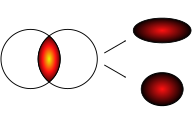
\includegraphics[width=\textwidth]{ellipticflow_viscous}};
      \node[anchor=north,xshift=2.5ex,yshift=-1ex,text width=10ex,text centered] at (fig.north) {small $\eta/s$ \\ large $v_2$};
      \node[anchor=south,xshift=2.5ex,yshift=1ex, text width=10ex,text centered] at (fig.south) {large $\eta/s$ \\ small $v_2$};
    \end{tikzpicture}

    \column{.55\textwidth}
    \begin{itemize}
      \item Observe experimental $v_n$.
      \item Run model with variable $\eta/s$.
      \item Constrain $\eta/s$ by matching $v_n$.
    \end{itemize}
  \end{columns}

  \bgs
  \centering
  \includegraphics[width=.8\textwidth]{osu} \\
  \flushright\tiny\vspace{-2ex}
  H.~Song, S.~A.~Bass, U.~Heinz, T.~Hirano and C.~Shen,
  PRL\ {\bf 106}, 192301 (2011).

\end{frame}




\begin{frame}{Extracting QGP properties}
  \vspace{1em}
  \begin{columns}
    \column{.45\textwidth}
    \begin{center}
      \bf Older work
    \end{center}
    \begin{itemize}
      \item Average calculations.
        \sms
      \item Vary only $\eta/s$, other parameters fixed.
        \sms
      \item Only several discrete values.
        \sms
      \item Qualitative constraints lacking uncertainty.
    \end{itemize}

    \column{.48\textwidth}
    \begin{center}
      \bf New projects
    \end{center}
    \begin{itemize}
      \item Event-by-event model.
        \sms
      \item Vary all salient parameters:  $\eta/s$, $\tau_0$, IC parameters, \ldots
        \sms
      \item Continuous parameter space.
        \sms
      \item Quantitative constraints including uncertainty.
    \end{itemize}
  \end{columns}
  
  \vspace{2em}
  \scriptsize
  See also: \\
  \begin{itemize}
    \item J.~Novak, K.~Novak, S.~Pratt, C.~Coleman-Smith and R.~Wolpert, \\ PRC \textbf{89}, 034917 (2014), arXiv:1303.5769 [nucl-th].
    \item R.~Soltz \textcolor{red}{REFERENCE}
  \end{itemize}

  %\tikz[overlay,remember picture] \node[xshift=-2ex,yshift=2ex] at (current page.center) {$\large\boldsymbol\Longrightarrow$};
  \tikz[overlay,remember picture] \node[xshift=-1.4ex,yshift=4ex] at (current page.center) {$\color{theme}\Large\boldsymbol\longrightarrow$};
  %\tikz[overlay,remember picture] \node[xshift=-1.4ex,yshift=13ex] at (current page.center) {$\color{theme}\Large\boldsymbol\longrightarrow$};
  %\tikz[overlay,remember picture] \node[xshift=-1.4ex,yshift=6ex] at (current page.center) {$\color{theme}\Large\boldsymbol\longrightarrow$};
  %\tikz[overlay,remember picture] \node[xshift=-1.4ex,yshift=-3ex] at (current page.center) {$\color{theme}\Large\boldsymbol\longrightarrow$};
  %\tikz[overlay,remember picture] \node[xshift=-1.4ex,yshift=-12ex] at (current page.center) {$\color{theme}\Large\boldsymbol\longrightarrow$};
  %\tikz[overlay,remember picture] \node at (current page.south east) {
  %  \scriptsize
  %  See also J.~Novak, K.~Novak, S.~Pratt, C.~Coleman-Smith and R.~Wolpert, PRC \textbf{89}, 034917, 2014, arXiv:1303.5769 [nucl-th].
  %};
\end{frame}



\section{Method}


\begin{frame}{Event-by-event model}
  \begin{center}
    \includegraphics[width=.8\textwidth]{evolution}
  \end{center}

  \begin{itemize}
    \item MC-Glauber \& MC-KLN initial conditions \\
      \hspace{1em} {\tiny H.-J.\ Drescher and Y.\ Nara, Phys.\ Rev.\ C {\bf 74}, 044905 (2006).}
    \item Viscous 2+1D hydro \\
      \hspace{1em} {\tiny H.\ Song and U.\ Heinz, Phys.\ Rev.\ C {\bf 77}, 064901 (2008).}
    \item Cooper-Frye hypersurface sampler \\
      \hspace{1em} {\tiny Z.\ Qiu and C.\ Shen, arXiv:1308.2182 [nucl-th].}
    \item UrQMD \\
      \hspace{1em} {\tiny S.\ Bass \emph{et.\ al.}, Prog.\ Part.\ Nucl.\ Phys.\  {\bf 41}, 255 (1998).} \\[-1ex]
      \hspace{1em} {\tiny M.\ Bleicher \emph{et.\ al.}, J.\ Phys.\ G {\bf 25}, 1859 (1999).}
  \end{itemize}

\end{frame}




\begin{frame}[label=atlas]{Experimental data}
  \begin{itemize}
    \item ATLAS event-by-event flow distributions $P(v_n)$ for $v_2,v_3,v_4$.
    \item Measure $\ve q_n = (\avg{\cos n\phi}, \avg{\sin n\phi})$ e-by-e; $v_n = |\ve q_n|$.
  \end{itemize}
  
  \vspace{3ex}

  \includegraphics[width=\textwidth]{atlas}
  \flushright \tiny ATLAS Collaboration, JHEP {\bf 1311}, 183 (2013).
\end{frame}




\begin{frame}[label=design]{Computer experiment design}
  \begin{itemize}
    \item Minimum \textbf{1000} events per set of input parameters and centrality class.
    \item \hyperlink{lhs}{\textbf{256} parameter points, varying 5 parameters simultaneously}
      \begin{itemize}
        \item Normalization
        \item IC-specific parameter
        \item Thermalization time $\tau_0$
        \item Viscosity $\eta/s$
        \item Shear relaxation time $\tau_\Pi$
      \end{itemize}
    \item \textbf{6} centrality classes 0--5\%, 10--15\%, \ldots, 50--55\%.
    \item \textbf{2} initial condition models.
  \end{itemize}

  %\begin{equation*}
  %  1000 \times 256 \times 6 \times 2 > 3 \text{ million events}
  %\end{equation*}
  %\begin{center}
  %  3 million hours $\sim$ 350 years
  %\end{center}
  \centering
  \vspace{2ex}
  \tikz\node[draw,thick,color=theme,text width=.6\textwidth,inner sep=2ex,text badly centered]{
    $1000 \times 256 \times 6 \times 2 > 3$ million events \\[.5ex] 3 million hours $\sim$ 350 years
  };
\end{frame}


\begin{frame}{Open Science Grid usage}
  \begin{center}
    \small
    \begin{tikzpicture}
      \node (fig) {\includegraphics[width=.8\textwidth]{osghours}};
      \node[anchor=south,yshift=-1ex,xshift=1.5ex] at (fig.north) {CPU hours per day};
      \node[anchor=south west,yshift=-1ex,xshift=1ex] at (fig.north west) {\small 250,000};
      \node[anchor=south west,yshift=1.5cm,xshift=.5cm] at (fig) {red = Me};
    \end{tikzpicture}
  \end{center}

  \vspace{-1em}

  \begin{itemize}
    \item Completed KLN design (1.5 million events) in two weeks.
    \item ${\sim}$4 million total $\rarr$ 0.55 $\mu\text{b}^{-1}$  (ATLAS:  7 $\mu\text{b}^{-1}$)
    \item Extensible to other projects.
  \end{itemize}
\end{frame}



\section{Results}


\begin{frame}[label=curves]{Model flow distributions}
  \vspace{2ex}
  \includegraphics{lhs-curves} \\

  Characterize distributions by
  \begin{itemize}
    \item Average flow $\avg{v_n}$
    \item Width of fluctuations (standard deviation) $\sigma_{v_n}$
    \item Relative width $\sigma_{v_n} / \avg{v_n}$
  \end{itemize}
\end{frame}



\begin{frame}{Flow results summary}
  \vspace{2ex}
  \centering
  \hspace{.46\textwidth}
  Glauber
  \hfill\tiny Lines: model, Points: ATLAS data \normalsize \\[.5ex]
  \includegraphics{lhs-cent-glb}
\end{frame}



\begin{frame}[label=emu]{Interpolating the parameter space}
  \begin{columns}
    \column{.6\textwidth}
    Gaussian process emulator
    \mds
    \begin{itemize}
      \item predict model output at arbitrary points in parameter space
        \mds
      \item quantitative uncertainty
    \end{itemize}

    \column{.4\textwidth}
    \hyperlink{gp}{\includegraphics[width=\textwidth]{gpr2}} \\[2ex]
    \raggedleft\tiny \emph{Gaussian Processes for Machine Learning}, \\ Rasmussen and Williams, 2006.
  \end{columns}

  \centering
  \vspace{1em}
  \tikz\node[draw,thick,color=theme,text width=.6\textwidth,inner sep=2ex,text badly centered]{
    Emulator predicts \textbf{1000 hours} worth of CPU time in \textbf{1 millisecond}
  };
\end{frame}



\begin{frame}{Emulator predictions}
  \centering\vspace{1ex}
  \hspace{.5ex} Glauber \\[1ex]
  \includegraphics{emu-cent-glb} \\
  \small\vspace{1ex}
  \begin{tabular}{rl}
    \textcolor{grey}{Colors} &
    \textcolor{vnbl}{$\boldsymbol{v_2}$}
    \textcolor{vngr}{$\boldsymbol{v_3}$}
    \textcolor{vnor}{$\boldsymbol{v_4}$} \\
    \textcolor{grey}{Lines} & $\eta/s = 0.04$, 0.08, 0.12, 0.16, top to bottom \\
    \textcolor{grey}{Points} & ATLAS data
  \end{tabular}
\end{frame}



\begin{frame}{Emulator predictions}
  \centering\vspace{1ex}
  \hspace{2.8ex} Glauber 20--25\% centrality \\[1ex]
  \includegraphics{emu-etas-glb} \\
  \small\vspace{1ex}
  \begin{tabular}{rl}
    \textcolor{grey}{Colors} &
    \textcolor{vnbl}{$\boldsymbol{v_2}$}
    \textcolor{vngr}{$\boldsymbol{v_3}$}
    \textcolor{vnor}{$\boldsymbol{v_4}$} \\
    \textcolor{grey}{Lines} & Glauber $\alpha = 0.06$, 0.12, 0.18, 0.24, bottom to top \\
    \textcolor{grey}{Bands} & ATLAS measurements
  \end{tabular}
\end{frame}



\begin{frame}{Flow results summary}
  \vspace{2ex}
  \centering
  \hspace{3ex} KLN \\[.5ex]
  \includegraphics{lhs-cent-kln}
\end{frame}



\begin{frame}{Emulator predictions}
  \centering\vspace{1ex}
  \hspace{1ex} KLN \\[1ex]
  \includegraphics{emu-cent-kln} \\
  \small
  \begin{tabular}{rl}
    \textcolor{grey}{Colors} &
    \textcolor{vnbl}{$\boldsymbol{v_2}$}
    \textcolor{vngr}{$\boldsymbol{v_3}$}
    \textcolor{vnor}{$\boldsymbol{v_4}$} \\
    \textcolor{grey}{Lines} & $\eta/s = 0.12$, 0.16, 0.20, 0.24, top to bottom \\
    \textcolor{grey}{Points} & ATLAS data
  \end{tabular}
\end{frame}



\begin{frame}{Emulator predictions}
  \centering\vspace{1ex}
  \hspace{3ex} KLN 20--25\% centrality \\[1ex]
  \includegraphics{emu-etas-kln} \\
  \small
  \begin{tabular}{rl}
    \textcolor{grey}{Colors} &
    \textcolor{vnbl}{$\boldsymbol{v_2}$}
    \textcolor{vngr}{$\boldsymbol{v_3}$}
    \textcolor{vnor}{$\boldsymbol{v_4}$} \\
    \textcolor{grey}{Lines} & KLN $\lambda = 0.10$, 0.15, 0.20, 0.25, bottom to top \\
    \textcolor{grey}{Bands} & ATLAS measurements
  \end{tabular}
\end{frame}


\begin{frame}{Intermission}
  \begin{itemize}
    \item Framework for massive event-by-event model-to-data comparison.
    \item Systematic model validation / exclusion.
      \begin{itemize}
        \item Glauber qualitatively describes data.
        \item KLN does not.
      \end{itemize}
    \item Repeat with more advanced models, especially initial conditions.
      \bgs
    \item Rigorously calibrate model to data \\
      $\rarr$ extract optimal parameters with uncertainty.
    \item Consider other observables, e.g.\ identified particle spectra, $dN_\text{ch}/dy$.
      \bgs
    \item \emph{Solve the finite-multiplicity problem.}
  \end{itemize}
\end{frame}


\section{Finite multiplicity}

\begin{frame}{Finite-multiplicity smearing}
  \def\obs{^\text{obs}}

  \begin{itemize}
    \item Observed flow smeared by finite multiplicity
      \begin{equation*}
        P(v_n\obs) = \int P(v_n\obs|v_n) P(v_n) \, dv_n
      \end{equation*}
      where $P(v_n\obs|v_n)$ is the response function.
    \item Pure statistical smearing $\rarr$ Bessel-Gaussian response
      \begin{equation*}
        P(v_n^\text{obs}|v_n) = \frac{v_n^\text{obs}}{\delta_{v_n}^2} e^{ -\frac{(v_n^\text{obs})^2 + (v_n)^2}{2\delta_{v_n}^2} }
          I_0 \pfrac{v_nv_n^\text{obs}}{\delta_{v_n}^2}.
      \end{equation*}
  \end{itemize}
\end{frame}


\begin{frame}{Finite-multiplicity correction}
  \vspace{1em}

  \begin{itemize}
    \item Fit flow distribution to Bessel-Gaussian
      \begin{equation*}
        P(v_n) = \frac{v_n}{\delta_{v_n}^2} e^{ -\frac{(v_n)^2 + (v_n^\text{RP})^2}{2\delta_{v_n}^2} }
          I_0 \pfrac{v_n^\text{RP}v_n}{\delta_{v_n}^2}.
      \end{equation*}
    \item Response function is also Bessel-Gaussian; determined by multiplicity.
    \item Keep $v_n^\text{RP}$, decrease width
      \begin{equation*}
        \delta_{v_n}^2 \rarr \delta_{v_n}^2 - 1/2M.
      \end{equation*}
  \end{itemize}
\end{frame}


\begin{frame}{Finite-multiplicity correction:  when it succeeds}
  \includegraphics[width=\textwidth]{fit_glb_20-25_200}

  \begin{itemize}
    \item Bessel-Gaussian fit is unambiguous:  log-likelihood has well-defined peak.
    \item Observed flow $\gg$ response function.
    \item $(\delta_{v_n}^2)^\text{obs} \gg 1/2M$.
  \end{itemize}
\end{frame}


\begin{frame}{Finite-multiplicity correction:  when it fails}
  \includegraphics[width=\textwidth]{fit_glb_20-25_65}

  \begin{itemize}
    \item Bessel-Gaussian fit is ambiguous:  log-likelihood has a long plateau.
    \item Observed flow $\sim$ response function.
    \item $(\delta_{v_n}^2)^\text{obs} \sim 1/2M$.
  \end{itemize}
\end{frame}


\begin{frame}{The fundamental problem}
  \begin{itemize}
    \item Finite-multiplicity smearing is not a one-to-one map.
    \item An observed flow distribution may have multiple possible origin distributions (within uncertainty).
  \end{itemize}
  \begin{columns}
    \column{.7\textwidth}
    \vspace{1em}
    \includegraphics{problem}
    \column{.3\textwidth}
    \hspace{-3em}
    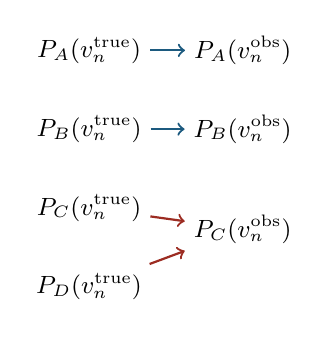
\begin{tikzpicture}
      \small
      \node              (l1) {$P_A(v_n^\text{true})$};
      \node[below of=l1] (l2) {$P_B(v_n^\text{true})$};
      \node[below of=l2] (l3) {$P_C(v_n^\text{true})$};
      \node[below of=l3] (l4) {$P_D(v_n^\text{true})$};
      \node[right of=l1, node distance=6em]              (r1) {$P_A(v_n^\text{obs})$};
      \node[right of=l2, node distance=6em]              (r2) {$P_B(v_n^\text{obs})$};
      \node[right of=l3, node distance=6em, yshift=-2ex] (r3) {$P_C(v_n^\text{obs})$};
      \draw[thick,->,theme] (l1) -- (r1);
      \draw[thick,->,theme] (l2) -- (r2);
      \draw[thick,->,themered] (l3) -- (r3);
      \draw[thick,->,themered] (l4) -- (r3);
    \end{tikzpicture}
  \end{columns}
\end{frame}


\begin{frame}{Possible solutions}
  \begin{itemize}
    \item Discard the bad points.
      \begin{itemize}
        \item Most are on edges of parameter space.
        \item $v_4$ is intrinsically small---many points would be lost.
      \end{itemize}
    \item Use a different fitting distribution.
      \begin{itemize}
        \item Correction algorithm more difficult.
        \item Still a poorly-defined inverse problem.
      \end{itemize}
    \item Don't use any distribution.
      \begin{itemize}
        \item Train an emulator (or other interpolator) to calculate true distribution moments given observed
          moments and multplicity.
        \item Still a poorly-defined inverse problem.
      \end{itemize}
    \item Bayesian unfolding---what ATLAS uses.
      \begin{itemize}
        \item Must bootstrap observed distribution to obtain sufficient statistics.
      \end{itemize}
    \item Oversample hydro.
      \begin{itemize}
        \item Need \emph{many} particles: smearing is $\sim 1/\sqrt M$.
        \item Significantly increases computation time and disk usage.
      \end{itemize}
  \end{itemize}
\end{frame}





\appendix

\def\backbutton#1{
  \tikz[remember picture,overlay]\node[anchor=south west] at (current page.south west) {\hyperlink{#1}{\footnotesize\color{theme}$\blacktriangleleft$}};
}

\begin{frame}[plain,noframenumbering]{}
  \centering
  \Large
  backup slides
\end{frame}


\begin{frame}[label=lhs]{Latin-hypercube sampling}
  \begin{itemize}
    \item Random set of parameter points.
    \item Maximizes CPU time efficiency.
    \item Skeleton of parameter space.
  \end{itemize}

  \bgs 

  \centering
  %\tikz\draw[thick] (0,0) rectangle node {LHS samples} (\textwidth,.35\textwidth);
  \includegraphics{lhs}
  %\includegraphics<2>{lhs2}

  \backbutton{design}
\end{frame}


\begin{frame}[label=gp]{Gaussian processes}

  %A Gaussian \emph{process} is a generalization of a Gaussian \emph{distribution}:  \\
  %instead of drawing random numbers, draw random functions. {\color{red} formal definition} \\[1.5em]

  \begin{itemize}
    %\item A Gaussian process is a stochastic process where each point is normally distributed.
    \item \emph{A Gaussian process is a collection of random variables, any finite number of which have a joint Gaussian distribution.}
    \item Instead of drawing variables from a distribution, functions are drawn from a process.
  \end{itemize}



  \begin{columns}[c]
    \column{.55\textwidth}
    Require a covariance function, e.g.
    \begin{equation*}
      \text{cov}(x_1,x_2) \propto \exp \biggl[ -\frac{(x_1 - x_2)^2}{2\ell^2} \biggr]
    \end{equation*}
    Nearby points correlated, distant points independent.

    \column{.45\textwidth}
    \includegraphics[width=\textwidth]{gpr1} \\[1ex]
    \raggedleft\tiny \emph{Gaussian Processes for Machine Learning}, \\ Rasmussen and Williams, 2006.
  \end{columns}

  \backbutton{emu}
\end{frame}


\begin{frame}{Generating Gaussian processes}
  \begin{columns}
    \column{.67\textwidth}
    \begin{itemize}
      \item Choose a set of input points $X_*$.
      \item Choose a covariance function, e.g.\
        \begin{equation*}
          k(x_i,x_j) = \exp[-(x_i-x_j)^2/2]
        \end{equation*}
        and create covariance matrix $K(X_*,X_*)$.
      \item Generate MVN samples (GPs)
        \begin{equation*}
          \vec f_* \sim \mathcal N[\vec 0,K(X_*,X_*)].
        \end{equation*}
    \end{itemize}

    \column{.33\textwidth}
    \includegraphics[width=\textwidth]{gpr1}
  \end{columns}

  \backbutton{emu}
\end{frame}


\begin{frame}{Gaussian process emulators}
  \begin{itemize}
    \item Prior:  the model is a Gaussian process.
    \item Posterior:  Gaussian process conditioned on model outputs.
  \end{itemize}

  %\sms

  \hspace{-5mm}
  \begin{tikzpicture}
    \draw[thick,->] (0,0) node[left] (prior) {\includegraphics[width=.41\textwidth]{gpr1}} -- 
    node[above] {Training} (1.8,0) node[right] (posterior) {\includegraphics[width=.41\textwidth]{gpr2}};
    \node[xshift=1.2ex] at (prior.north) {Prior};
    \node[xshift=1.5ex] at (posterior.north) {Posterior};
    %\node[align=right,anchor=east] at (posterior.south east) {\tiny Rasmussen and Williams, \emph{Gaussian processes for machine learning}.};
  \end{tikzpicture}
  
  %\sms

  \begin{itemize}
    \item Emulator is a fast surrogate to the actual model.
      \begin{itemize}
        \item More certain near calculated points.
        \item Less certain in gaps.
      \end{itemize}
  \end{itemize}

  \backbutton{emu}
\end{frame}


\begin{frame}{Training the emulator}
  \begin{itemize}
    \item Make observations $\vec f$ at training points $X$.
    \item Generate conditioned GPs
        \begin{align*}
          \vec f_* | X_*,X,\vec f &\sim \mathcal N[K(X_*,X)K(X,X)^{-1}\vec f, \\
          &\qquad {} K(X_*,X_*) - K(X_*,X)K(X,X)^{-1}K(X,X_*)].
        \end{align*}
  \end{itemize}

  \centering

  \begin{tikzpicture}
    \draw[thick,->] (0,0) node[left] (prior) {\includegraphics[width=.35\textwidth]{gpr1}} -- (1,0) node[right] (posterior) {\includegraphics[width=.35\textwidth]{gpr2}};
    \node[xshift=1.2ex] at (prior.north) {Prior};
    \node[xshift=1.5ex] at (posterior.north) {Posterior};
  \end{tikzpicture}

  \backbutton{emu}
\end{frame}






\end{document}
